\chapter{Kernel Methods}

\section{Introduction}

$K:\mathcal{X}\times \mathcal{X}\rightarrow \mathbb{R}$称为$\mathcal{X}$上的\textbf{Kernels}。

\begin{mdframed}
    \begin{theorem}
        (\textbf{Mercer's condition})\hspace{0.4em} 令$\mathcal{X}\subset \mathbb{R}^N$是一个紧集\footnote{$\mathcal{X}$是紧集,则存在有限个开覆盖},$K:\mathcal{X}\times \mathcal{X}\rightarrow \mathbb{R}$是一个对称连续函数,则
        \begin{equation}
            K(x,x')=\sum_{n=0}^{\infty} \lambda_n\phi_n(x)\phi_n(x'),\ a_n>0 \ is \ eigenvalue
        \end{equation}

        当且仅当$\forall c\in L^2(\mathcal{X})$,下面的条件成立
        \begin{equation}
            \int\int_{\mathcal{X}\times\mathcal{X}}c(x)c(x')K(x,x')dxdx'\geqslant 0
        \end{equation}
    \end{theorem}
\end{mdframed}

\textbf{proof.}\hspace{0.5em} 

$\Box$

\textsl{Mercer’s condition}是核方法中的一个重要概念,尤其在支持向量机(SVM)和核函数的理论中
起着关键作用。它为一个函数能否作为合法的核函数提供了数学判据,保证了凸性从而保证可以取到全局最小值。合法的核函数用于将数据从低维空间映射到高维空间,在高维空间中可以更加容易地进行线性分割。

\section{Positive definite symmetric kernel}

$K:\mathcal{X}\times \mathcal{X}\rightarrow \mathbb{R}$称为\textbf{正定核}(\textsl{positive definite symmetric,PDS}),当对于任何$\{x_1,\cdots,x_m\}\subseteq \mathcal{X}$,矩阵
\begin{equation}
    \mathbf{K}=\left[ K(x_i,x_j) \right]_{ij}\in \mathbb{R}^{m\times m}
\end{equation}

是半正定对称矩阵,即$\forall \mathbf{c}=(c_1,\cdots,c_m)^T\in \mathbb{R}^{m\times 1}$,
\begin{equation}
    \mathbf{c}^T\mathbf{Kc}=\sum_{i,j=1}^{n}c_ic_jK(x_i,x_j)\geqslant 0
\end{equation}

\begin{example}
    (\textbf{Polynomial Kernels})\hspace*{0.5em} 对任意常数$c>0$,一个$d$维多项式核定义为
    \begin{equation}
        \forall\ \mathbf{x},\mathbf{x}'\in \mathbb{R}^N,\ \ \ K(\mathbf{x},\mathbf{x}')=(\mathbf{x}\cdot \mathbf{x}'+c)^d
    \end{equation}

    多项式核将输入空间映射到更高维度的空间。作为一个例子,$N=2$的输入空间,二阶多项式多项式对应于下面的内积
    \begin{equation}
        \forall\ \mathbf{x},\mathbf{x}'\in \mathbb{R}^2,\ \ K(\mathbf{x},\mathbf{x}')=(x_1x_1'+x_2x_2'+c)^2=
        \left[
            \begin{array}{c}
            x^2_1 \\
            x^2_2 \\
            \sqrt{2}x_1x_2\\
            \sqrt{2c}x_1\\
            \sqrt{2c}x_2\\
            c
        \end{array}\right]^T
        \left[
            \begin{array}{c}
                x'^2_1 \\
                x'^2_2 \\
                \sqrt{2}x'_1x'_2\\
                \sqrt{2c}x'_1\\
                \sqrt{2c}x'_2\\
                c
            \end{array}
        \right]
    \end{equation}

    可以看到这是维度为$6$的内积。
    \begin{figure}[H]
        \centering
        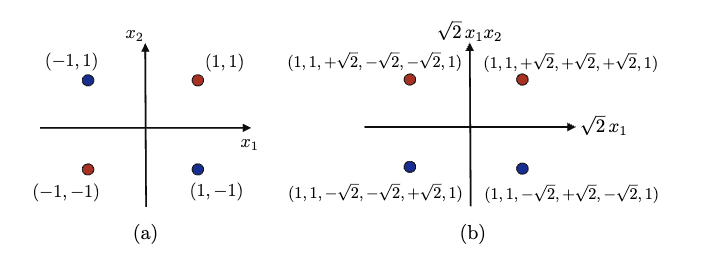
\includegraphics[scale=0.6]{figures/ploynaimal-kernel.png}
        \caption{异或问题}
    \end{figure}

\end{example}

\begin{example}
    (\textbf{Gaussian Kernels})\hspace*{0.5em} 对于任意的常数$\sigma>0$,\textbf{高斯核}\textsl{(Gaussian kernel)}或者称\textbf{径向基函数}\textsl{(radial basis function, RBF)}定义为
    \begin{equation}
        \forall\ \mathbf{x},\mathbf{x}'\in \mathbb{R}^N,\ \ \ K(\mathbf{x},\mathbf{x}')=\exp\left(-\frac{\Vert \mathbf{x}'-\mathbf{x}\Vert}{2\sigma^2}\right)
    \end{equation}

    高斯核是应用中使用最为频繁的。我们将会证明高斯核是\textsl{PDS}核并且它能通过正规化的方法构造
    \begin{equation}
        K':(\mathbf{x},\mathbf{x}')\rightarrow \exp((\frac{(\mathbf{x}\cdot \mathbf{x}')^n}{\sigma^2}))
    \end{equation}
\end{example}
\begin{example}
    (\textbf{Sigmoid Kernels})\hspace*{0.5em} 对于任意的实数$a,b\geqslant 0$,一个\textsl{Sigmoid kernel}定义为
    \begin{equation}
        \forall\ \mathbf{x},\mathbf{x}'\in \mathbb{R}^N,\ \ \ K(\mathbf{x},\mathbf{x}')=\tanh\left(a(\mathbf{x}\cdot \mathbf{x}')+b\right)
    \end{equation}
\end{example}

\section{Reproducing kernel Hilbert Space}

\begin{mdframed}
  \begin{lemma}
    (\textbf{Cauchy-Schwarz inequality for PDs kernels})\hspace{0.5em} 令$K$为一个\textsl{PDS kernel},则对于任意的$x,x'\in \mathcal{X}$
    \begin{equation}
        K(x,x')\leqslant K(x,x)K(x',x')
    \end{equation}
  \end{lemma}  
\end{mdframed}

\textbf{proof.}\hspace*{0.5em} 考虑矩阵
\begin{equation}
    \mathbf{K}=\left(
        \begin{array}{cc}
            K(x,x) & K(x,x') \\
            K(x',x) & K(x',x') \\ 
        \end{array}
    \right)
\end{equation}

根据定义,$K$是\textsl{PDS}核,则$\mathbf{K}$是\textsl{SPSD}对于所有的$x,x'\in \mathcal{X}$。$mathbf{K}$的特征值的积$det(\mathbf{K})$必须是非负的,因此
$K(x',x)=K(x,x')$,我们有
\begin{equation}
    det(\mathbf{K})=K(x,x)K(x',x')-K(x,x')^2>0
\end{equation}

$\Box$

\begin{mdframed}
    \begin{theorem}
        令$K:\mathcal{X}\times \mathcal{X}\rightarrow \mathbb{R}$是一个\textsl{PDS}核,则存在一个\textsl{Hilbert Space}$\ \mathbb{H}$以及$\Phi:\mathcal{X}\rightarrow \mathbb{H}$,使得
        \begin{equation}
            \forall x,x'\in \mathcal{X},\ \ K(x,x')=\left<\Phi(x),\Phi(x')\right>
        \end{equation}

        $\mathbb{H}$有如下名为\textbf{再生}\textsl{(Reproducing)}的性质
        \begin{equation}
            \forall h\in \mathbb{H},\forall x\in \mathcal{X},\ h(x)=\left< h,K(x,\cdot) \right>
        \end{equation}

        $\mathbb{H}$称为\textbf{再生核希尔伯特空间}(\textsl{reproducing kernel Hilbert Space,RKHS})。
    \end{theorem}
\end{mdframed}

\textbf{proof.}\hspace{1em} 对于任意的$x\in \mathcal{X}$,定义$\Phi:\mathcal{X}\rightarrow \mathbb{R}^\mathcal{X}$
\begin{equation}
    \forall\ x,x'\in \mathcal{X},\ \ \ K(x,x')=\left< \Phi(x),\Phi(x') \right>
\end{equation}

定义$\mathbb{H}_0$为$\Phi(x)$的线性组合的集合
\begin{equation}
    \mathbb{H}_0:=\left\{ \sum_{i\in I}a_i\Phi(x_i)\ :\ a_i\in \mathbb{R},x_i\in \mathcal{X},|I|<\infty \right\}
\end{equation}

在$\mathbb{H}_0\times \mathbb{H}_0$中引入一个运算$\left< \cdot,\cdot \right>$,对于所有的$f,g\in \mathbb{H}_0$,其中$f=\sum_{i\in I} a_i\Phi(x_i)$,$g=\sum_{j\in J} b_j\Phi(x_j')$
\begin{equation}
    \left<f,g\right>=\sum_{i\in I,j\in J} a_i b_j K(x_i,x_j')=\sum_{j\in J}b_j f(x_j')=\sum_{i\in I}a_j g(x_i)
\end{equation}

根据定义自然$\left< \cdot,\cdot \right>$是一个对称算子。最后两个等号展示$\left< f,g \right>$并不依赖于$f$和$g$的形式,以及显示$\left< \cdot,\cdot \right>$的双线性。对于任意$f=\sum_{i\in I} a_i\Phi(x_i)\in \mathbb{H}_0$,由于
$K$是一个$PDS$核,我们有
\begin{equation}
    \left<f,f\right>=\sum_{i,j} a_i a_j K(x_i,x_j)\geqslant 0
\end{equation}

因此,$\left< \cdot,\cdot \right>$是一个双线性半正定型。更一般地,对于任意的$f_1,\cdots,f_m\in \mathbb{H}_0$,$c_1,c_2,\cdots,c_m\in \mathbb{R}$,
\begin{equation}
    \sum_{i,j=1}^{m}c_ic_j\left< f_i,f_j \right>=\left< \sum_{i=1}^{m}c_if_i,\sum_{j=1}^{m}c_jf_j \right>\geqslant 0
\end{equation}

因此,$\left< \cdot,\cdot \right>$是$\mathbb{H}_0$上的$PDS$核,因此,对于任意的$f\in \mathbb{H}_0$和任意的$x\in \mathcal{X}$,根据\textsl{Cauchy-Schwarz inequality},我们写为
\begin{equation}
    \left< f,\Phi(x) \right>^2\leqslant \left<f,f\right>\left<\Phi(x),\Phi(x)\right>
\end{equation}

根据再生性:对于任意的$f=\sum_{i\in I}a_i\Phi(x_i)\in \mathbb{H}_0$,根据$\left<\cdot,\cdot\right>$的定义
\begin{equation}
    \forall x\in \mathcal{X},\ \ f(x)=\sum_{i\in I}a_i K(x_i,x)=\left<f,\Phi(x)\right>
\end{equation}

因此,对于所有的$x\in \mathcal{X}$,$|f(x)|^2\leqslant \left<f,f\right>K(x,x)$。这意味着$\left<\cdot,\cdot\right>$定义了一个$\mathbb{H}_0$上的内积,因此$\mathbb{H}_0$称为了一个\textsl{pre-Hilbert space}。
下面只要对$\mathbb{H}_0$能完备化就能形成成$\mathbb{H}$。根据\textsl{Cauchy-Schwarz}不等式,对$\forall x\in \mathcal{X}$,$f\mapsto \left<f,\Phi(x)\right>$是\textsl{Lipschitz}的,因此是连续的,因此$\mathbb{H}_0$在$\mathbb{H}$中稠密。

$\Box$

\subsection*{\textsl{Normlized PDS Kernels}}

\begin{mdframed}
    \begin{lemma}
        令$K$是一个\textsl{PDS kernel},则$K$的规范核$K'$也是\textsl{PDS kernel}.
    \end{lemma}
\end{mdframed}

\subsection*{\textsl{PDS Kernels Closure Properies}}

\begin{mdframed}
    \begin{theorem}
        \textsl{PDS kernel}在和、积、张量积、逐点极限下是闭集,且可以展开成幂级数
        \begin{equation}
            \sum^{\infty}_{n=0}a_nx^n,\ a_n\geqslant 0\ for\ \forall n\in \mathbb{N}
        \end{equation}
    \end{theorem}
\end{mdframed}

\section{Kernel-Based Algorithms}

\subsection*{\textsl{SVMs with PDS kernels}}

由于一个\textsl{PDS}核暗示着定义一个内积,我们能延伸\textsl{SVM}
\begin{equation}
    \begin{aligned}
        & \max_{\alpha}\sum_{i=1}^{m}\alpha_i-\frac{1}{2}\sum_{i,j=1}^{m}\alpha_i\alpha_j y_i y_j K(x_i,x_j) \\
        & subject\ to:0\leqslant \alpha_i\leqslant C \wedge \sum_{i=1}^{m}\alpha_iy_i=0,\ i\in [m]
    \end{aligned}
\end{equation}

假设的解$h$能写成
\begin{equation}
    h(x)=sgn\left(\sum_{i=1}^{m}\alpha_iy_iK(x_i,x)+b\right)
\end{equation}

其中$b=y_i-\sum_{j=1}^{m}\alpha_jy_jK(x_j,x_i),\forall x_i,0<\alpha_i<C$。我们能将优化问题重新写成向量的形式,通过$K$的核矩阵$\mathbf{K}$
\begin{equation}
    \begin{aligned}
        & \max_{\alpha}\ 2\ \mathbf{1}^T\mathbf{\alpha}-(\mathbf{\alpha}\circ \mathbf{y})^T\mathbf{K}(\mathbf{\alpha}\circ \mathbf{y})\\
        & subject\ to:\mathbf{0}\leqslant \mathbf{\alpha}\leqslant \mathbf{C}\wedge \mathbf{\alpha}^T\mathbf{y}=0
    \end{aligned}
\end{equation}

\subsection*{\textsl{Representer theorem}}

\begin{mdframed}
    \begin{theorem}
        令$K:\mathcal{X}\times\mathcal{X}\rightarrow\mathbb{R}$是一个\textsl{PDS}核,$\mathbb{H}$对应$RKHS$,则,对于任意的不减函数$G:\mathbb{R}\rightarrow \mathbb{R}$和任意的损失函数$L:\mathbb{R}^m\rightarrow \mathbb{R}\cup \{+\infty\}$,优化问题
        \begin{equation}
            \arg\min_{h\in \mathbb{H}} F(h)=\arg\min_{h\in \mathbb{H}} G(\Vert h\Vert_\mathbb{H})+L(h(x_1),\cdots,h(x_m))
        \end{equation}

        存在一个解的形式为
        \begin{equation}
            h^*=\sum_{i=1}^{m}\alpha_i K(x_i,\cdot)
        \end{equation}

        如果$G$在先前假设是增函数名,则任何解都是这样的形式。
    \end{theorem}
\end{mdframed}

\textbf{proof.}\hspace{1em} 

$\Box$

\subsection*{Learning guarantees}

\begin{mdframed}
    \begin{theorem}
        (\textbf{Rademacher complexity of kernel-based hypotheses}) 令$K:\mathcal{X}\times \mathcal{X}\rightarrow \mathbb{R}$是一个\textsl{PDS}核,$\Phi:\mathcal{X}\rightarrow \mathbb{R}$是一个关于$K$的特征映射。令$S\subseteq \{x:K(x,x)\leqslant r^2\}$是一个尺寸为$m$的例子,令
        $\mathcal{H}=\{x\mapsto \left<\mathbf{w},\Phi(x)\right>:\ \Vert \mathbf{w}\Vert_{\mathbb{H}}\leqslant \Lambda,\exists \Lambda>0\}$,则
        \begin{equation}
            \hat{\mathcal{R}}_S(\mathcal{H})\leqslant \frac{\Lambda\sqrt{Tr[\mathbf{K}]}}{m}\leqslant \sqrt{\frac{r^2\Lambda^2}{m}}
        \end{equation}
    \end{theorem}
\end{mdframed}

\textbf{proof.}\hspace{1em} 

$\Box$

\begin{mdframed}
    \begin{corollary}
        (\textbf{Margin bounds for kernel-based hypotheses})令$K:\mathcal{X}\times \mathcal{X}\rightarrow\mathbb{R}$是一个\textsl{PDS}核,其中$r^2=\sup_{x\in \mathcal{X}}K(x,x)$,令$\Phi:\mathcal{X}\rightarrow \mathbb{H}$是一个关于$K$的特征映射,令$\mathcal{H}=\{\mathbf{x}\mapsto \mathbf{w}\cdot \Phi(x):\Vert \mathbf{w}\Vert_\mathbb{H}\leqslant \Lambda,\exists \Lambda\geqslant 0\}$。固定$\rho>0$,则对于任意的$\delta>0$
        \begin{equation}
            R(h)\leqslant \hat{R}_{S,p}(h)+2\sqrt{\frac{r^2\Lambda^2/\rho^2}{m}}+\sqrt{\frac{\log \frac{1}{\delta}}{2m}} \\
        \end{equation}
        \begin{equation}
            R(h)\leqslant \hat{R}_{S,p}(h)+2\sqrt{\frac{Tr[\mathbf{K}]\Lambda^2/\rho^2}{m}}+3\sqrt{\frac{\log \frac{2}{\delta}}{2m}} \\
        \end{equation}
    \end{corollary}
\end{mdframed}


\section{Negative definite symmetric kernels}

\begin{define}
    (\textbf{Negative definite symmetric kernels, NDS}) 一个核$K:\mathcal{X}\times \mathcal{X}\rightarrow \mathbb{R}$称为\textbf{负定对称}\textsl{(Negative-definite symmetric,NDS)},如果这是一个对称核并且$\forall\ (x_1,\cdots,x_m)\subseteq \mathcal{X}$以及$\mathbf{c}\in \mathbb{R}^{m\times 1}$,满足$\mathbf{1}^T\mathbf{c}=0$下面的关系成立
    \begin{equation}
        \mathbf{c}^T\mathbf{K}\mathbf{c}\leqslant 0
    \end{equation}
\end{define}

明显地,如果$K$是\textsl{PDS},则$-K$是\textsl{NDS},但反过来一般来说并不成立。

\begin{example}
    (\textbf{Squared distance——NDS kernel})\hspace{0.5em} 
\end{example}

\section{Sequence Kernel}

\subsection*{\textsl{Weighted transducers}}

\subsection*{\textsl{Rational kernel}}